%%%%%%%%%%%%%%%%%%%%%%%%%%%%%%%%%%%%%%%%%%%%
% 
% Last edits: Nov 9, 2016
%%%%%%%%%%%%%%%%%%%%%%%%%%%%%%%%%%%%%%%%%%%%

\documentclass[12pt]{article}
\usepackage{natbib}
\usepackage[letterpaper, margin=1.1in]{geometry}
\usepackage{graphicx}
\usepackage[table,xcdraw]{xcolor}
\usepackage{wrapfig}
\usepackage{enumitem}
\setlist[enumerate]{itemsep=0mm}
\usepackage{multirow}
\usepackage{lscape}
\usepackage{caption}
\usepackage{subcaption}
\usepackage{float}
\usepackage{hyperref}


\begin{document}
\noindent{Alexandra Pulwicki \\ \today}

\begin{center}
\Large \textbf{Methods\\ Data Processing}
\end{center}


\section*{Overview}
This section documents the process of going from raw data to processed and consolidated data that will be used for analysis in subsequent components of the project. A description of the various scripts used to process this data is provided and the final data structure is outlined.


\tableofcontents
\pagebreak


%%%%
\section{Data Processing}
%%%%
This section documents the process of going from raw data to processed and consolidated data that will be used for analysis in subsequent components of the project. A description of the various scripts used to process this data is provided and the final data structure is outlined.

To run the entire data processing framework first ensure your desired outcome in reflect in the `OPTIONS.m' script and then run both `OPTIONS.m' and `MAIN.m'.


\subsection{Linear and Curvilinear Transects}

Snow depth measurements along the linear and curvilinear transects were taken at locations a certain distance from marked waypoints. Since only the coordinates of the waypoints (WP) were recorded, the measurement coordinates needed to be estimated. The measurement locations were assumed to be 10, 20, and 30 m behind the marked WP, in a straight line between the marked WP and the previous WP. In cases with only two observers, locations were assumed to be 10 and 20 m behind the marked WP. For the first marked WP of a pattern, it was assumed that the locations were along the same line as that between the first and second WPs. The following methodology was used to determine measurement locations (each step corresponds with a section of the Matlab code `MeasurementLocations.m'): 
\begin{enumerate}
\item Waypoint (WP) locations were exported from the GPS units using the BaseCamp program. They were then imported to QGIS and exported with UTM coordinates. This file was then used in the Matlab script and is entitled `GlacierWP\_UTM.xlsx'. 
\item In order to obtain the measurement locations for the first WPs of each pattern, an ``imaginary'' WP was created that was along the line between the first and second WPs, but located ahead of the first WP. These waypoints were then inserted into the original data. 
\item A set of 1000 equally spaced points was created along a straight line between each set of subsequent of WPs (including the ``imaginary'' WPs from the previous step) using the function linspaceNDim.m created by Steeve Ambroise and downloaded from the MathWorks File Exchange. The Euclidean distance between these interpolated points and the marked WP was then calculated and the points with distances closest to the assumed separation between observers were retained. The final matrix has the easting and northing of each measurement location and is labelled with the marked WP and a decimal that corresponds to the relative observer (e.g. label 45.2 means that the location was determined from the marked WP \#45 and is 20 m behind this WP because it is the second observer). 
\end{enumerate}

The data recorded by each observer in the field books was transcribed to a spreadsheet format and then imported and processed in Matlab according to the following steps (each step corresponds with a section of the Matlab code `Import\_Transect.m'):
\begin{enumerate}
\item A spreadsheet was created with a sheet for data from each field book (SD\#1, SD\#2, SD\#3, and SWEDepth). For each reference WP there were values for all snow depth measurements and their quality (1 for good, 0 for bad), comments written, field book name, glacier name, observer, pattern, and date collected.  
\item The quality, comments, book name, glacier name, observer, pattern, and date entries were categorized. This allows for efficient grouping and data searching in future analysis.
\item The depth data was then assigned the corresponding measurement location UTM from the `MeasurementLocations.m' script. This was done by matching the WP number from the field books and that of the marked WPs and then assigning the coordinates from the WP ending with .1 to depths recorded in book SD\#1, and likewise for the remaining books. The matrices for each set of observations were then made to be the same dimensions by inserting empty cells for WPs where no data was recorded in that set of observations. 
\item The data was then arranged in a structure variable (called SD) with rows corresponding to each book (e.g. row 1 is data from book SD\#1) and columns corresponding to the various types of data (e.g. depth values or glacier category). For example, the matrix with the glacier category for each value recorded in the book SD\#1 can be accessed with `SD(1).glacier'.
\end{enumerate}

Subsets of the transect data can be pulled using the function `pulldata.m'. The function is called with \texttt{pulldata(data, book, glacier, person, pattern, quality, format)}. Here, \texttt{data} is the full SD structure, \texttt{book, glacier, person, and pattern} are all strings that refer to desired categories, \texttt{quality} differentiates between good (1), bad (0), or `all' data, and \texttt{format} specifies the formatting of the full depth matrix as being either a column vector ('skinny') or a matrix with depth values for one WP in a single row. 


\subsection{Zigzag}

Data from zigzag measurements, which includes the measured snow depth and the distance of that measurement from the previous measurement or vertex, was transcribed to a spreadsheet. The data were then processed using the following procedure (each step corresponds with a section of the Matlab code `Import\_Zigzag.m'):
\begin{enumerate}
\item Data were imported into Matlab.
\item Descriptive data, including glacier name, zigzag zone label, reference vertex, data quality, observer name, date collected, and book name were categorized.
\item A structure was created with the depth and categorical data.
\item The distance of each measurement point from it's reference vertex was then calculated. These locations were assumed to be a cumulative sum of distances in a straight line between two subsequent vertices. Two options exist for the location of the reference vertex:
 	\begin{enumerate}
	\item Option 1 calculates the distance of each point from the UTM coordinates of the reference vertex.
	\item Option 2 calculates the distance of each point from the end of the previous line of measurements. Since the total distance measured with the avalanche probe did not always equal the distance between vertices (likely due to error in GPS units), this option takes the reference for each line to be from the end of the previous line. The coordinates of the vertices were used for the start of each `Z' shape (ZZ01 and ZZ05).
	\end{enumerate}
\item The final processing step involves removing bad quality data, obtaining the index for the start of each zigzag (needed for future analysis), as well as converting snow depth to snow water equivalent (SWE) based on the density calculated from the average SWE values measured with the Federal Sampler in each zigzag (if Option 2 is selected for that section).  
\end{enumerate}

\subsection{Density}

The density data from snowpit and Federal Sampler measurements were compiled into a spreadsheet and the density from each measurement was calculated and summarized in a spreadsheet. 

Integrated snow density was calculated from snowpit measurements. This was done by multiplying the measured density from each wedge sample by the depth of the sample and summing these values. A density of 917 kg m$^{-3}$ was applied to ice layers and a density of 600 kg m$^{-3}$ was applied to layers that were described as `hard' and were too difficult to sample. To determine the error in estimating integrated snow density, the values of ice density, ice thickness, and the `hard` layer density was varied between 700 and 917 kg m$^{-3}$, $\pm$ 1 cm, and 500 and 600 kg m$^{-3}$, respectively.  A summary of density values and ranges is shown in Table \ref{tab:density_stats}.

\begin{table}[b!]
\centering
\caption{Mean and standard deviation (std) of snow density (kg m$^{-3}$) as well as number of measurements (n) of snow density measured on study glaciers in snowpits and using a Federal Sampler. }
\label{tab:density_stats}
\begin{tabular}{ccccccc}
 & \multicolumn{3}{c}{\textbf{Snowpits}} & \multicolumn{3}{c}{\textbf{Federal Sampler}} \\
\multirow{-2}{*}{\textbf{Glacier}} & Mean & Std & n & Mean & Std & n \\ \hline
\textbf{Glacier 4} & 348 & 13 & 3 & 355 & 18 & 7 \\
\textbf{Glacier 2} & 333 & 26 & 4 & 286 & 34 & 7 \\
\textbf{Glacier 13} & 349 & 26 & 3 & 316 & 40 & 17 \\
\rowcolor[HTML]{EFEFEF} 
\textbf{All} & 342 & 26 & 10 & 318 & 42 & 31
\end{tabular}
\end{table}

Density values determined from Federal Sampler measurements were filtered based on quality and then averaged for each measurement location. Measurements that were deemed to be unrepresentative of the local snow pack, which included measurements where the inner core length was less than 70\% of the snow depth or where density values were exceptionally high (e.g. 490 kg m$^{-3}$), were marked as bad quality data. The data was processed in Matlab as follows (each step corresponds with a section of the Matlab code `Import\_Density.m'): 
\begin{enumerate}
\item Data were imported into Matlab and only good quality data were kept. Indices for data subsets (e.g. only density values from snowpits) were identified manually. 
\item The mean density, standard deviation, and number of good measurements was calculated for the zigzag locations (Federal Sampler).
\item The mean density, standard deviation, and number of good measurements was calculated for the snowpit locations (Federal Sampler) and combined in a matrix with the corresponding snowpit derived density values.
\item A structure with the processed data was created.
\end{enumerate}

The final version of the `Density' structure includes five fields:
\begin{itemize}
\item[]\texttt{Density.snowpit} includes the density data from the snowpit. Columns correspond to snowpit label, assumed density, easting, northing, elevation, minimum density, maximum density, snow depth.
\item[]\texttt{Density.pitANDtube} includes data from locations where measurements were taken in a snowpit and with a Federal Sampler. Columns correspond to snowpit label, Federal  Sampler mean density, standard deviation, minimum values, maximum values, and number of observations, snowpit derived density, site elevation, minimum snowpit density, and maximum snowpit density.
\item[]\texttt{Density.tube} includes Federal Sampler data. Columns correspond to location label, density mean, standard deviation, minimum, maximum, number of good quality observations, easting, northing, elevation, and depth. 
\item[]\texttt{Density.zigzagtube} includes density values at each zigzag location estimated using a Federal Sampler. Columns correspond to zigzag label, mean density, standard deviation, number of observation, and site elevation. 
\item[]\texttt{Density.SWEdepth} is a summary of all the snow depth and Federal Sampler derived density data. Columns correspond to location label, mean probe depth, depth measured by the Sampler, and snow density estimated using the Federal Sampler. 
\end{itemize}

\subsection{Snow water equivalent (SWE)}

The conversion of measured snow depth to snow water equivalent (SWE) proved to be challenging because snow density was not measured at all locations where snow depth was measured. This meant that the density measurements need to be interpolated. There are a number of different methodologies for doing this interpolation within the glaciology literature and that ones that were chosen for this project can be seen in Figure \ref{fig:SWEoptions}. Since there was no true justification for choosing one option over the other, a selection of methods applicable to the study were chosen. There were three main methods that were used. The first assumed a uniform spatial distribution of SWE \citep[e.g.]{McGrath2015, Elder1991}. A subset of this method was to use the mean density over the entire Donjek Range was used (same value for all glaciers) and a second subset used a mean density for each glacier (different value for all glaciers). The second and third methods involved spatially variable density values. One of these methods involved doing an elevation regression with the measured density values to interpolate between measurement locations and the other one used an inverse-distance weighted mean for interpolation. Since the snowpit derived density and Federal Sampler derived density had no relationship, the two density datasets were kept separate. This mean that for each density interpolation option, there were two outputs. In the end, there were eight different interpolations of density that would be carried forward throughout the study, which allows for a range of SWE estimates to be made.

{
\begin{wrapfigure}{r}{\textwidth} 
	\centering
	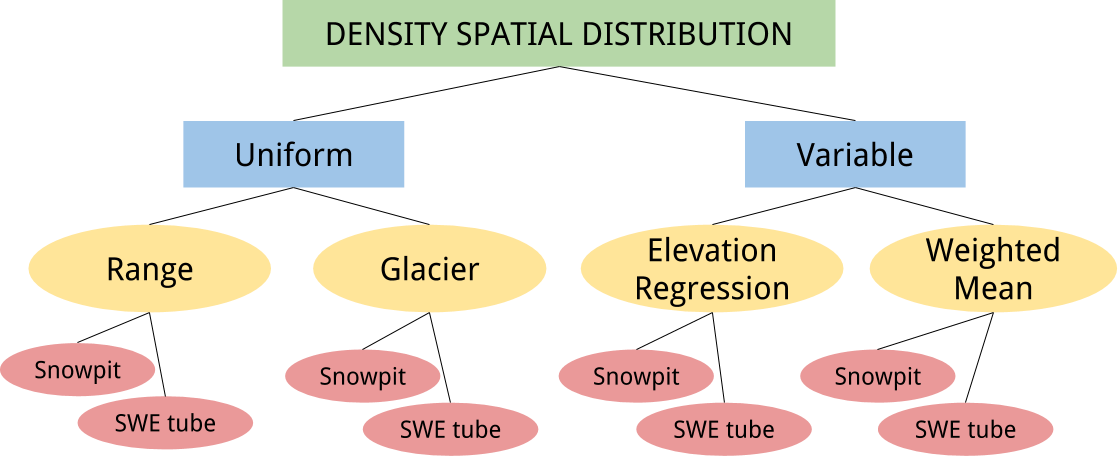
\includegraphics[width = \textwidth]{SWEoptions.png}\\
	\caption{Relationship between various ways to interpolate between density measurements for the calculation of SWE.}
	\label{fig:SWEoptions}
\end{wrapfigure}
}

The final SWE values were calculated in Matlab using the following steps (this corresponds to the script `Import\_SWE.m'):
\begin{enumerate}
\item Data from transects, zigzags, and extra measurements was complied into a single structure called `SWE'.
\item The elevation of each measurement location according to the SPOT5 DEM was found in QGIS and the data was imported to Matlab and assigned to each value.
\item The density values were interpolated and assigned to each value
	\begin{itemize}
	\item[Option 1] Does not calculate SWE and keeps the depth value.
	\item[Option 2] Calculates the mean density of all snowpit measurements.
	\item[Option 3] Calculates the mean density of all Federal Sampler measurements.
	\item[Option 4] Calculates the mean density for each glacier using the snowpit measurements. 
	\item[Option 5] Calculates the mean density for each glacier using the Federal Sampler measurements. 
	\item[Option 6] Calculates the slope and intercept of the snowpit densities with elevation for each glacier using the `fit' function and then uses this to determine density for all elevations associated with each measurement location.
	\item[Option 7] Calculates the slope and intercept of the Federal Sampler densities with elevation for each glacier using the `fit' function and then uses this to determine density for all elevations associated with each measurement location.
	\item[Option 8] Determines the distance between each measurement location and each snowpit the calculates the inverse-distance weight. For each measurement location, each snowpit density is then multiplied by its weight and these values are added together and divided by the sum of all weights. 
	\item[Option 9] Determines the distance between each measurement location and each Federal Sampler the calculates the inverse-distance weight. For each measurement location, each Federal Sampler density is then multiplied by its weight and these values are added together and divided by the sum of all weights. 
	\end{itemize}
\end{enumerate}
To chose which SWE calculation option to use (or to cycle through all options) the value of \texttt{options.DensitySWE} to changed to the option number.

The final version the 'SWE' structure includes three rows that correspond to Glacier 4, 2, and 13 and ten fields that include information about each individual SWE estimate. The fields are: \texttt{book} (field book where they are written), \texttt{comments} (any comments noted by observer), \texttt{density} (the density value used to calculate SWE), \texttt{depth} (mean depth measured at each sampling location, $n=3$ usually), \texttt{glacier} (which glacier the measurement was taken on), \texttt{label} (measurement point reference label - for transects this is the waypoint number and relative position, for other measurements this is a label associated with shape and location), \texttt{pattern} (pattern that the measurement is a part of), \texttt{person} (initials of observer), \texttt{swe} (estimated SWE value), and \texttt{utm} (the easting and northing for the measurement location as well as the DEM elevation). To access the SWE values for Glacier 2, one would type \texttt{SWE(2).swe}. 

The `SWE' structure includes all data that was collected for each glacier. If there is a need to remove the zigzag data or keep only the zigzag data, the script `ZigzagRemoval.m' can be run. Set the option for including or excluding zigzag data in the script `OPTIONS.m'.




\bibliography{/home/glaciology1/Documents/MastersDocuments/MastersLit}
\bibliographystyle{igs}

\end{document}